\documentclass[margin=1mm]{standalone}
\usepackage{tikz}

\begin{document}
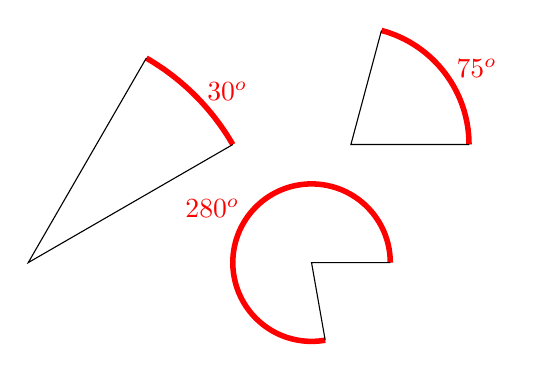
\begin{tikzpicture}
	
	\def\startangle{30};
	\def\endangle{60};
	\def\raio{3};
	
	\node[] (origem) at (0,0) {};
	
	\draw[red, line width=2pt, anchor=south west] (0,0) arc (\startangle:\endangle:\raio) node [midway, right, yshift=0.05cm, xshift=0.0 cm] {30$^o$};
	\draw[black, anchor=south west] (0,0) -- ++(\startangle+180:\raio) -- +(\endangle:\raio);


	\def\startangleb{0};
	\def\endangleb{75};
	\def\raiob{1.5};
	
	\draw[red, line width=2pt, anchor=south west] (3,0) arc (\startangleb:\endangleb:\raiob) node [midway, right, yshift=0.05cm, xshift=0.0 cm] {\endangleb$^o$};
	\draw[black] (3,0) -- ++(\startangleb+180:\raiob) -- +(\endangleb:\raiob);
	
	\def\startanglec{0};
	\def\endanglec{280};
	\def\raioc{1.00};
	
	\draw[red, line width=2pt, anchor=south west] (2,-1.5) arc (\startanglec:\endanglec:\raioc) node [midway, left, yshift=0.05cm, xshift=0.0 cm] {\endanglec$^o$};
	\draw[black, anchor=south west] (2,-1.5) -- ++(\startanglec+180:\raioc) -- +(\endanglec:\raioc);	

\end{tikzpicture}
\end{document}
